\documentclass[a4paper,11pt]{scrartcl}

\usepackage[ngerman]{babel}
% uncomment or modify according to your operating system
% \usepackage[applemac]{inputenc} % european characters can be used (Mac OS)
% \usepackage[latin1]{inputenc}
\usepackage{ucs} % fuer deutsche Sonderzeichen unter Linux
\usepackage[utf8x]{inputenc} %fuer deutsche Sonderzeichen unter Linux
% \usepackage[utf8]{inputenc} fuer deutsche Sonderzeichen unter Windows
\usepackage[T1]{fontenc}
\usepackage{graphicx}
\usepackage{fullpage}
\usepackage{latexsym}
\usepackage{amssymb}
\usepackage{amsmath}
\usepackage{ifthen}
\usepackage{listings}
\usepackage{color}
\usepackage{hyperref}
\usepackage{cite}

\definecolor{dkgreen}{rgb}{0,0.6,0}
\definecolor{gray}{rgb}{0.5,0.5,0.5}
\definecolor{mauve}{rgb}{0.58,0,0.82}
\lstset{ %
  language=Matlab,                % the language of the code
  basicstyle=\small,              % the size of the fonts that are used for the code
  numbers=left,                   % where to put the line-numbers
  numberstyle=\tiny\color{gray},  % the style that is used for the line-numbers
  stepnumber=1,                   % the step between two line-numbers. If it's 1, each line
                                  % will be numbered
  numbersep=5pt,                  % how far the line-numbers are from the code
  backgroundcolor=\color{white},      % choose the background color. You must add \usepackage{color}
  showspaces=false,               % show spaces adding particular underscores
  showstringspaces=false,         % underline spaces within strings
  showtabs=false,                 % show tabs within strings adding particular underscores
  frame=single,                   % adds a frame around the code
  rulecolor=\color{black},        % if not set, the frame-color may be changed on line-breaks within not-black text (e.g. commens (green here))
  tabsize=2,                      % sets default tabsize to 2 spaces
  captionpos=b,                   % sets the caption-position to bottom
  breaklines=true,                % sets automatic line breaking
  breakatwhitespace=false,        % sets if automatic breaks should only happen at whitespace
  title=\lstname,                   % show the filename of files included with \lstinputlisting;
                                  % also try caption instead of title
  keywordstyle=\color{blue},          % keyword style
  commentstyle=\color{dkgreen},       % comment style
  stringstyle=\color{mauve},         % string literal style
  escapeinside={\%*}{*)},            % if you want to add LaTeX within your code
  morekeywords={end,sortrows}               % if you want to add more keywords to the set
}


% Abkuerzungen fuer haeufige Befehle wie z.B. griechische Buchstaben
\newcommand{\N}{\mathbb{N}}
\newcommand{\Z}{\mathbb{Z}}
\newcommand{\R}{\mathbb{R}}
\newcommand{\C}{\mathbb{C}}
\newcommand{\F}{\mathcal{F}}
\newcommand{\La}{\mathcal{L}}
\newcommand{\de}{\delta}
\newcommand{\e}{\varepsilon}
\newcommand{\la}{\lambda}
\newcommand{\p}{\varphi}
\newcommand{\al}{\alpha}
\newcommand{\be}{\beta}
\newcommand{\om}{\omega}
\newcommand{\Om}{\Omega}
\newcommand{\ta}{\tau}
\newcommand{\g}{\gamma}
\newcommand{\HE}{\mathbb{H}}
\newcommand{\E}{\mathbb{E}}
\newcommand{\vG}{\varGamma}
\newcommand{\s}{\sigma}

\begin{document}

\subject{Modeling \& Simulation}
\title{SIR Model - Mass Tests}

\publishers{Betreuer: Martin Bicher }


\author{
Christian Göth \and
Christian Sallinger \and
Florian Schager \and
Paul Winkler
}

\maketitle

\section*{Abstract}

In 2020 the COVID-19 pandemic caused worldwide suffering and deaths and the
whole world is waiting for a vaccine. In winter 2020/2021 countries in Europe
came up with the idea of executing nationwide mass tests to reduce the number
of unconfirmed cases. This strategy should serve as an alternative to
lockdown measures that force people to reduce their contacts.
In this project we want to contrast these alternatives qualitatively and quantitatively
by constructing a modified SIR Model to simulate the spread of the disease.
With our model we want to answer the question:
How many days of lockdown are necessary with different strategies of mass-testing?


\newpage

\tableofcontents

\newpage

\section{Model Description}

Our model is based on the classical SIR Model by Kermack and McKendrick,
but in addition to the standard compartments Susceptible, Infectious, Recovered
we introduce an extra Exposed compartment between the Susceptible and the Infectious.
Furthermore we split the Infectious compartment into two seperate compartments:
Confirmed and Unconfirmed. \\
In our model we assume, that the persons in the Confirmed compartment are in
quarantine and do not contribute to the infection rate anymore.



Causal Loop Diagram: \\


Stock and Flow Diagram: \\

\section{Modell}

\subsection{Unterkapitel 2.1}
\label{sec:Unterkapitel21}
 Literaturquellen müssen im File \textit{References.bib} defniniert werden und können
 dann hier einfach mittels \verb|\cite{QUELLE}| referenziert werden.

 Empfehlenswerte Literatur zum Thema \emph{Kontinuierliche Simulation} ist z.B.:
 \cite{CK06}.

\subsubsection{Unterkapitel 2.1.1}
 Verwenden Sie die Latex Distribution Mik\TeX (unter Windows) bzw. \TeX  Live (unter Linux)
 und als IDE z.B. \emph{\TeX nicCenter}\footnote{\url{http://www.texniccenter.org/}} (unter Windows)
 oder z.B. \emph{Kile}\footnote{\url{http://kile.sourceforge.net}} (unter Linux).

\subsection{Unterkapitel 2.2}
Hier möchte ich auf Kapitel \ref{sec:Unterkapitel21} Bezug nehmen.

\section{Implementation}

\subsection{Source Code}

Als nächstes fügen wir Source-Code aus einer Datei ein:

 \lstinputlisting[
 basicstyle=\tiny,       % the size of the fonts that are used for the code
 frame=single,
 numbers=left,                   % where to put the line-numbers
 numberstyle=\tiny,      % the size of the fonts that are used for the line-numbers
 stepnumber=1,                   % the step between two line-numbers. If it's 1, each line
                                 % will be numbered
 caption={Die Funktion {\itshape polar2cartesian}.},
 label=SRC:polar2cartesian] {./SourceCode/BeispielCode.m}

Listing \ref{SRC:polar2cartesian} zeigt den Source-Code der Funktion \verb polar2cartesian .
Hierbei wurde ganz am Beginn des .tex-Files mittels \verb \lstset  angegeben, dass es sich
bei dem in Folge einzufügenden Code um Matlab-Code handelt. Aus diesem Grund sind die
Schlüsselwörter so schön eingefärbt.

Source Code ohne Datei:
\begin{lstlisting}[
 basicstyle=\footnotesize, % the size of the fonts that are used for the code
 frame=single,
 language=c++,
 numbers=left,             % where to put the line-numbers
 escapeinside={//*}{*//},  % for line labeling
 caption={Definition der Klasse \texttt{InOutputVector}.},
 label=src:InOutputVector_defs]
 class InOutputVector:public std::vector<InOutput> {
   public:
     int untreated_entry_changes;

     InOutputVector() {            //* \label{lnbr:InOutput_constructor} *//
       untreated_entry_changes = 0;
     }
     void setAt(int c,double val,double t) {
       if(true==(*this)[c].already_treated) {
         untreated_entry_changes++;
       }
       (*this)[c].set(val,t);
     }
     double* treatAt(int c,double val) {
       if(false==(*this)[c].already_treated) {
         untreated_entry_changes--;
       }
       return((*this)[c].treat());
     }
     void treatAll() {
       for(int i=0; i<this->size(); i++){
         (*this)[i].already_treated = true;
       }
       untreated_entry_changes=0;
     }
 };
\end{lstlisting}

In Zeile \ref{lnbr:InOutput_constructor} in Listing \ref{src:InOutputVector_defs} ist der Kontruktor der Klasse
\verb|InOutputVector| implementiert.

\section{Simulation Results}

Tabelle \ref{tab:ParA} zeigt den verwendeten Parametersatz.
\begin{table}[!h]
{\small%
\newcommand{\mc}[3]{\multicolumn{#1}{#2}{#3}}
\begin{center}
\begin{tabular}{|c|c|c|c|c|c|c|c|c|c|c|}
 \hline
 $t_{end}$ [s] & $X_0$ [m]    & $V_0$ [m/s]  & $d$ & relTol & absTol & Refine & maxdist & Tol\\
 \hline
      100      & $\binom{0}{2}$ & $\binom{2}{0}$ &  1  & 1e-3   &  1e-6  &    8   &     2   &  $\binom{1e-3}{1e-6}$ \\
 \hline
\end{tabular}
\end{center}
}%
\caption{Parametersatz A.}
\label{tab:ParA}
\end{table}

\begin{figure}[!ht]
 \centering
 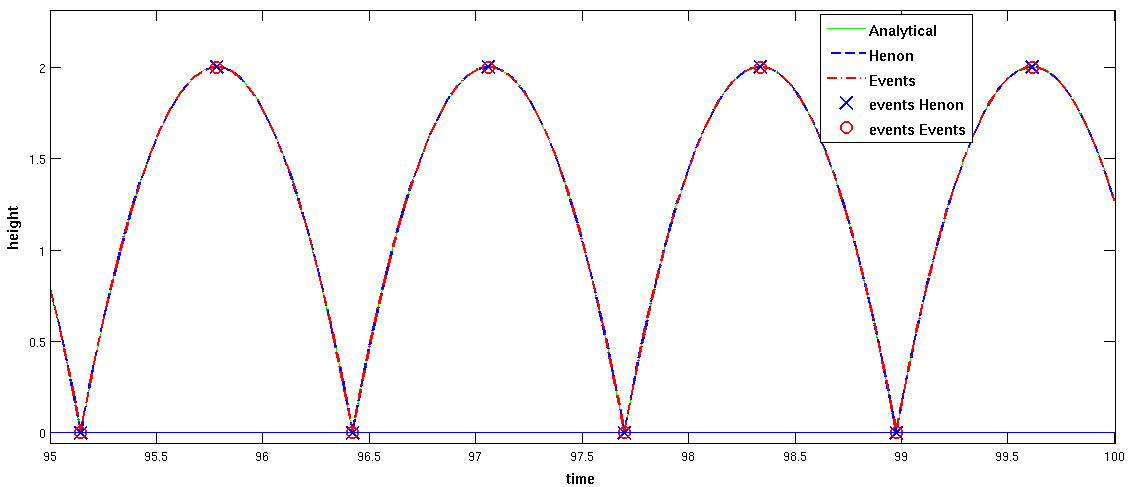
\includegraphics[width=\textwidth]{./Bilder/bBheightode23last5Sec.png}
 % bBheightode23last5Sec.png: 1130x487 pixel, 90dpi, 31.89x13.75 cm, bb=0 0 904 390
 \caption{Simulationsergebnisse unter Verwendung von Parametersatz A.}
 \label{fig:Bild2}
\end{figure}

\section{Conclusio}
Es wurde gezeigt, wie in Latex einzeilige, mehrzeilige, nummerierte und nicht nummerierte
Formeln erzeugt werden können, sowie wie auf Formeln verwiesen werden kann und wie Matrizen
erzeugt werden können. Weiters wurde gezeigt wie auf verwendete Literatur verwiesen werden kann,
wie Source-Code eingefügt werden kann und wie auf einzelne Zeilen im Source Code verwiesen werden kann.
Das Einfügen von Bildern und das Erzeugen von Tabellen wurde ebenfalls demonstriert.

Die grobe Struktur Ihres Projektprotokolls soll wie in diesem Dokument sein.

Zusammenfassend ist zu sagen, dass Sie die meisten \LaTeX{} - Befehle die Sie für ihr Protokoll
brauchen werden, hier in diesem Template finden sollten. Es wird Ihnen aber trotzdem nicht erspart
bleiben, sich einmal etwas genauer mit der \LaTeX{} Syntax auseinander zu setzen. Literatur und Foren
zu \LaTeX{}  sind im Internet ausreichend vorhanden.

\newpage

\bibliographystyle{alpha}
\bibliography{References}

\end{document}
